\documentclass[11pt]{amsart}
\usepackage{geometry}      
\geometry{letterpaper}                  
\usepackage{graphicx}
\usepackage{amssymb}
\usepackage{epstopdf}
\usepackage[applemac]{inputenc}
\usepackage{amsmath}
\usepackage{amssymb}
\usepackage{amsthm}
\usepackage{enumerate}
\usepackage{tikz}
\usetikzlibrary{positioning}
\tikzset{>=stealth}

\geometry{verbose,a4paper,tmargin=25mm,bmargin=25mm,lmargin=25mm,rmargin=25mm}

\providecommand{\norm}[1]{\lVert #1 \rVert}
\providecommand{\abs}[1]{\lvert #1 \rvert}
\providecommand{\ip}[2]{\langle #1, #2\rangle}

\DeclareGraphicsRule{.tif}{png}{.png}{`convert #1 `dirname #1`/`basename #1 .tif`.png}
\newtheorem{defi}{Definition}
\newtheorem{satz}{Satz}
\newtheorem{bsp}{Beispiel}

\title{�bungsaufgaben Algebraische Topologie - Serie 4}
\author{Franz Patzig}


\begin{document}
\maketitle

\section{Aufgabe}
F�r je zwei komplexe abelsche Gruppen K und L definieren wir einen Komplex Hom(K,L) in dem wir f�r jedes $n \in \mathbb{Z}$ setzen
\begin{equation*}
\text{Hom(K,L)}_n := X_{k \in \mathbb{Z}} \text{Hom(}\text{K}_k, \text{K}_{k+n})
\end{equation*}
d.h. ein Element von Hom(K,L) ist eine Familie
\begin{equation*}
f = \{f_k : K_k \to L_{k+n} \}_{k \in \mathbb{Z}}
\end{equation*}
von Gruppenhomomorphismen. Der Rand von f sei durch
\begin{equation*}
\partial_n(f) := \{\partial_n^L \circ f_k - (-1)^n f_{k-1} \circ \partial_n^K \}_{k \in \mathbb{Z}}
\end{equation*}
gegeben.

\textbf{(i) Zu zeigen:} Auf diese Weise ist tats�chlich ein Komplex definiert.
\begin{defi}[Komplex K] Ein Komplex K ist eine Familie $\{\partial_n:K_n \to K_{n-1} \}_{n \in \mathbb{Z}}$ von aufeinanderfolgenden Homomorphismen mit der Eigenschaft, dass die Zusammensetzung von je zwei aufeinanderfolgenden Homomorphismen Null ist:
\begin{equation}
\label{komplex}
\partial_{n-1} \circ \partial_n = 0
\end{equation}
\end{defi}
Damit m�ssen wir \ref{komplex} zeigen mit $\partial_n((f_n)_{n \in \mathbb{Z}}) = (\partial_n^L \circ f_n - 1 \cdot (-1)^n f_{n-1} \circ \partial_n^K)_{n \in \mathbb{Z}}$.
\begin{eqnarray*}
\partial_{n-1} \circ \partial_n =& \partial_{n-1}((f_n)_{n \in \mathbb{Z}}) \circ \partial_n((f_n)_{n \in \mathbb{Z}}) \\
=& (\partial_{n-1}^L \circ f_n - 1 \cdot (-1)^{n-1} f_{n-1} \circ \partial_{n-1}^K) \circ (\partial_n^L \circ f_n - 1 \cdot (-1)^n f_{n-1} \circ \partial_n^K) \\
=& 0 
\end{eqnarray*} 

\textbf{(ii) Zu beschreiben:} Zyklen $\text{Z}_0\text{Hom(K,L)}$.
\begin{defi}[Zyklen] 
\begin{equation}
\text{Z}_n \text{K := Ker}(\partial_n)
\end{equation}
\end{defi}
Was bedeutet es, wenn jeder Eintrag 0 ist, also auf der rechten Seite nur 0en stehen?

\textbf{(iii) Zu beschreiben:} R�nder $\text{B}_0\text{Hom(K,L)}$.
\begin{defi}[R�nder]
\begin{equation}
\text{B}_n \text{K := Im}(\partial_{n+1})
\end{equation}
\end{defi}
Linke Seite gleich 0.

\section{Aufgabe}

\section{Aufgabe}
\textbf{Zu zeigen:} F�r eine kurze exakte Sequenz
\begin{center}
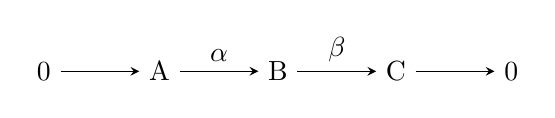
\begin{tikzpicture}
    % set up the nodes
    \node (E) at (0,0) {0};
    \node[right=of E] (F) {A};
    \node[right=of F] (G) {B};
    \node[right=of G] (H) {C};
    \node[right=of H] (I) {0};
    % draw arrows and text between them
    \draw[->] (E)--(F) node [midway,above] {};
    \draw[->] (F)--(G) node [midway,above] {$\alpha$};
    \draw[->] (G)--(H) node [midway,above] {$\beta$};
    \draw[->] (H)--(I) node [midway,above] {};
\end{tikzpicture}
\end{center}
von abelschen Gruppen sind die folgenden Bedingungen �quivalent.
\begin{enumerate}[(i)]
\item Die Sequenz zerf�llt, d.h. es handelt sich bis auf Isomorphie um die Sequenz

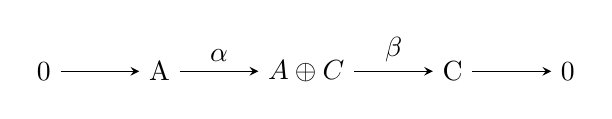
\begin{tikzpicture}
    % set up the nodes
    \node (E) at (0,0) {0};
    \node[right=of E] (F) {A};
    \node[right=of F] (G) {$A \oplus C$};
    \node[right=of G] (H) {C};
    \node[right=of H] (I) {0};
    % draw arrows and text between them
    \draw[->] (E)--(F) node [midway,above] {};
    \draw[->] (F)--(G) node [midway,above] {$\alpha$};
    \draw[->] (G)--(H) node [midway,above] {$\beta$};
    \draw[->] (H)--(I) node [midway,above] {};
\end{tikzpicture} 
mit $\alpha (a) = (a,0)$ und $\beta (a,c) = c$.\\
\item Es gibt einen zu $\alpha$ linksinversen Homomorphismus. \\
\item Es gibt einen zu $\beta$ rechtsinversen Homomorphismus. \\
\item Es gibt Homomorphismus: $a': B \to A$ und $b': C \to B$ mit $\alpha' \circ \alpha = \text{id}$, $\beta \circ \beta' = \text{id}$, $\alpha \circ \alpha' + \beta' \circ \beta =�\text{id}$. \\
\end{enumerate}

\textbf{(i) $\to$ (ii):} Wir zeigen als erstes, dass es einen Isomorphismus $\varphi : A \oplus C \to B$ mit $\varphi(a,0) = f(a)$ und $h \circ \varphi(a,c) = c$ gibt. Wir definieren $\varphi(a,c) = f(a) + r(c)$. Dann kommutiert das Diagramm
\begin{center}
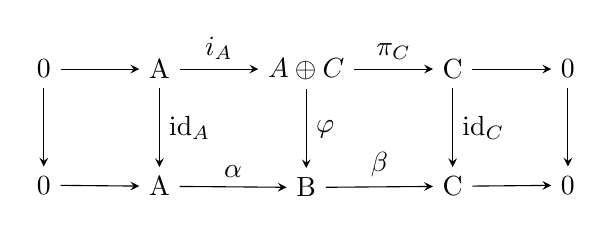
\begin{tikzpicture}
    % set up the nodes
    \node (E) at (0,0) {0};
    \node[right=of E] (F) {A};
    \node[right=of F] (G) {$A \oplus C$};
    \node[right=of G] (H) {C};
    \node[right=of H] (I) {0};
    
    \node[below=of E] (J) {0};
    \node[below=of F] (K) {A};
    \node[below=of G] (L) {B};
    \node[below=of H] (M) {C};
    \node[below=of I] (N) {0};
    % draw arrows and text between them
    \draw[->] (E)--(F) node [midway,above] {};
    \draw[->] (F)--(G) node [midway,above] {$i_A$};
    \draw[->] (G)--(H) node [midway,above] {$\pi_C$};
    \draw[->] (H)--(I) node [midway,above] {};
     \draw[->] (J)--(K) node [midway,above] {};
    \draw[->] (K)--(L) node [midway,above] {$\alpha$};
    \draw[->] (L)--(M) node [midway,above] {$\beta$};
    \draw[->] (M)--(N) node [midway,above] {};
      \draw[->] (E)--(J) node [midway,above] {};
    \draw[->] (F)--(K) node [midway,right] {$\text{id}_A$};
    \draw[->] (G)--(L) node [midway,right] {$\varphi$};
    \draw[->] (H)--(M) node [midway,right] {$\text{id}_C$}; 
        \draw[->] (I)--(N) node [midway,above] {}; 

\end{tikzpicture}
\end{center}
und das F�nferlemma zeigt, dass $\varphi$ ein Isomorphismus ist. Setzt man $r(c) = \varphi(0,c)$ so erkennt man, dass die Sequenz spaltet. Es sei $\psi = \varphi^{-1}$. Dann erhalten wir $r$ durch $r(b) = (\pi_A \circ \psi)(b)$. \\

\textbf{(ii) $\to$ (iii):} Sei $r: B \to A$ eine \textit{Retraktion} von $\alpha$. Wir definieren dann eine Abbildung $s: C \to B$ durch $c \mapsto b - \alpha \circ r(b)$. F�r ein $b \in \beta^{-1}(c)$. Dabei verwenden wir, dass f�r $b, b' \in \beta^{-1}(c)$ gilt $b - b' \in \text{Her}(\beta) = \text{Im}(\alpha)$, d.h. $\alpha \circ r(b - b') = b - b'$, also $b - \alpha \circ r(b) = b' - \alpha \circ r(b')$. Sofort pr�ft man jetzt nach, dass $s$ ein Homomorphismus ist und dass $\beta \circ s = \text{id}_T$ gilt. \\

\textbf{(iii) $\to$ (ii):} Sei $s: C \to B$ ein \textit{Schnitt} zu $\beta$. Wir definieren einen Homomorphismus $r : B \to A$ durch die Vorschrift $ b \mapsto \alpha^{-1}(b - s \circ \beta(b))$. Wir verwenden hier erstens, dass durch $b \mapsto m - s \circ \beta(b)$ ein Homomorphismus $ B \to B$ definiert wird, zweitens, dass wegen $\beta(m - s \circ \beta(b)) = \beta(b) - \beta \circ s \circ \beta(b) = \beta(b) - \beta(b) = 0$ jeweils $ b - s \circ \beta(b) \in \text{Ker}(\beta) = \text{Im}(\alpha)$, und drittens, dass $\alpha$ injektiv ist. F�r $a \in A$ folgt wegen der Injektivit�t von $\alpha$ und $s$, dass $r \circ \alpha(a) = \alpha^{-1}(\alpha(a) - s \circ \beta(\alpha(a))) = \alpha^{-1}(\alpha(a)) - \alpha^{-1}(s(0)) = a$. Damit gilt: $r \circ \alpha = \text{id}_A$.\\

\textbf{(iii) $\to$ (iv):}
\end{document}  